\chapter{The Graph-Simplex Correspondence}
\label{chap:correspondence}

\chapterquote{The right understanding of any matter and a misunderstanding of the same matter do not wholly exclude each other.
}{Franz Kafka, \emph{The  Trial}}

\chapterquote{Why, sometimes I've believed as many as six impossible things before  breakfast.}{Lewis Carroll, \emph{Alice's Adventures in Wonderland}}

In this chapter we introduce the graph simplex correspondence and explore its mathematical foundations and properties. While the focus of this dissertation is the bijective relationship between graphs and simplices, we begin by introducing the more general relationship between matrices and convex polytopes. The correspondence between graphs and simplices will then follow as a consequence. 


\section{Convex Polyhedra of Matrices}
\label{sec:correspondence_polyhedra_matrices}
Here we introduce the polytope associated with a given matrix. Let $\M\in \R^{n\times n}$ be PSD and admitting of the eigendecomposition $\M=\sum_{i=1}^d \lambda_i \eig_i\eig_i^\tp$ for some $d\leq n$ (i.e., $\M$ has eigenvalue zero with multiplicity $n-d$) where the eigenvectors $\{\eig_i\}_{i=1}^d $ are orthonormal. Writing out the eigendecomposition as 
\begin{equation*}
\M=\Eig_M\Eval_M\Eig_M^\tp=(\Eig_M\Eval_M^{1/2})(\Eig_M\Eval_M^{1/2})^\tp,
\end{equation*}
with $\Eig_M = (\vp_1,\dots,\vp_d)$, $\Eval_M=\diag(\lambda_1,\dots,\lambda_d)$ (note the respective absences of $\vp_{d+1},\dots,\vp_n$ and $\lambda_{d+1},\dots,\lambda_n$), suggests that we might consider $\Eval_M^{1/2}\Eig_M$ as a vertex matrix, thus $\M$ as a gram matrix. 
Inorexably compelled by this intuition, define the vertices $\sv_1,\dots,\sv_n$ given by the columns of $\Eval_M^{1/2}\Eig_M^\tp$, i.e.,  
\begin{equation*}
    \sv_i = (\Eval_M^{1/2}\Eig_M^\tp) (\cdot,i) = (\eig_1(i)\lambda_1^{1/2}, \eig_2(i)\lambda_2^{1/2},\dots,\eig_d(i)\lambda_d^{1/2})^\tp\in \R^d,
\end{equation*}
where we emphasize that the vertex vector will have real entries since $\lambda_j> 0$ for all $j\in[d]$ since  $\M$ is PSD. We may now define the \emph{polytope of the matrix $\M$} as the polytope given by their convex hull:
\begin{equation*}
\pol_\M\equiv \conv(\sv_1,\dots,\sv_n).
\end{equation*}
Letting $\Sv=\Sv(\pol_\M)=(\sv_1,\dots,\sv_n)\in \R^{d\times n}$ be the matrix whose $i$-th column is the $i$-th vertex $\sv_i$---henceforth called the \emph{vertex matrix of $\P_M$}---we see that 
$ \Sv=\Eval_M^{1/2}\Eig_M^\tp=(\Eig_M\Eval^{1/2})^\tp$, and 
\begin{equation*}
    \Sv^\tp \Sv=(\Eig\Eval^{1/2}) (\Eig\Eval^{1/2})^\tp = \Eig \Eval\Eig^\tp =\M.
\end{equation*}
Observe that the polytope $\splx(\M)$ is $d$-dimensional, i.e., its vertices span a $d$-dimensional subspace, since
$\rank(\Sv)=\rank(\Sv^\tp \Sv)=\rank(\M)=d$, 
where we've employed Lemma \ref{lem:rank(QtQ)} and the fact that $\M$ has rank $d$ due to its eigendecomposition. We thus conceptualize $\P_M$ as a polytope in $\R^d$. 

\begin{remark}
	The ordering of the non-zero eigenvalues did not enter our considerations when defining $\P_M$. Let us consider re-ordering the indices; take $\tau:[d]\to[d]$ to be any permutation and $\{\sv_i^\tau\}$ be the vertices as they would be defined under the ordering given by $\tau$. Hence $\sv_i^\tau(j) = \vp_{\tau^{-1}(j)}(i)\lambda_{\tau^{-1}(j)}^{1/2}$. The pairwise distances between these vertices then obey 
	\begin{equation*}
	\norm{\sv_i^\tau-\sv_k^\tau}_2^2 = \sum_{j=1}^d \lambda_{\tau^{-1}(j)} (\vp_{\tau^{-1}(j)}(i)-\vp_{\tau^{-1}(j)}(k))^2 = \sum_{j=1}^d \lambda_{j} (\vp_{j}(i)-\vp_{j}(k))^2 = \norm{\sv_i-\sv_j}_2^2,
	\end{equation*}
	since $\tau$ is a bijection, hence summing over $\tau^{-1}(j)$ yields the same result as summing from 1 to $d$. 
	Therefore, we see that the polytopes $\conv(\sv_1^\tau,\dots,\sv_n^\tau)$ and  $\conv(\sv_1,\dots,\sv_n)$ are congruent. In fact, since they share the same centroid they are simply rotations of one another. 
\end{remark}


\subsection{The Inverse Polytope} 
\label{sec:inverse_polytope}
Given that we can associate a polytope with the matrix $\M$, it is natural to wonder about the relationship between this polytope and that associated to $\M^{-1}$ if $\M$ if invertible, or with its pseudoinverse $\M^+$ more generally. As illustrated in Section \ref{sec:background_pseudoinverse}, with the eigendecompition of $\M$ as above, we can write  the pseudoinverse as 
\[\M^+=\sum_{i=1}^d \lambda_i^{-1} \eig_i\eig_i^\tp = \Eig_M \Eval_M^{-1/2}\Eig_M.\]
We can thus associated with $\M^+$ a polytope $\pol_{\M^+}$, which has as its vertex matrix $\Sv(\pol_{\M^+})=(\Eig\Eval^{-1/2})^\tp$; that is, the vertices $\{\sv_i^+\}$ of $\pol_{\M^+}$ are defined by 
$\sv_i^+(j)=\eig_j(i)/\lambda_j^{1/2}$. We call $\pol_{\M^+}$ the \emph{inverse polytope of $\M$}. 

Let us observe several properties of the relationship between $\P_M$ and $\P_{M^+}$. In what follows we drop the subscript $M$ from the eigenvalue and eigenvector matrix. Note that because of the orthogonality relationships among eigenvectors of $\M$, 
\[\Eig^\tp \Eig = \begin{pmatrix}
\la \vp_1,\vp_1\ra & \dots & \la \vp_1,\vp_d \ra \\
\vdots & \ddots & \vdots \\
\la \vp_d,\vp_1\ra & \dots & \la \vp_d,\vp_d\ra
\end{pmatrix} = \I_d.\]
Consequently, 
\begin{equation*}
\M^+\M = \Eig\Eval\Eig^\tp \Eig\Eval^{-1}\Eig^\tp = \Eig\Eval\Eval^{-1}\Eig^\tp = \Eig\Eig^\tp,
\end{equation*}
and similarly $\M\M^+= \Eig\Eig^\tp$. As it happens, the vertex matrices of $\P_M$ and $\P_M^+$ satisfy the same pseudoinverse relation: 
\begin{equation*}
\Sv^\tp\Sv^+ = \Eig \Eval^{1/2}\Eval^{-1/2}\Eig^\tp = \Eig\Eig^\tp, 
\end{equation*}
and $(\Sv^+)^\tp\Sv = \Eig\Eig^\tp$. Using the properties of the relationship between a matrix and its pseudoinverse immediately yields the following result. 

\begin{lemma}
\label{lem:vertex_matrices_pseudoinverse}
	Let $\Sv=\Sv(\M)$ and $\Sv^+=\Sv(\M^+)$ by the vertex matrices of $\P_M$ and $\P_{M^+}$ where $\M$ is a real and symmetric matrix. The matrices $\Sv^\tp\Sv^+$ and $(\Sv^+)^\tp\Sv$ are equal and moreover 
	\begin{enumerate}
		\item[(i).] act as the orthogonal projection onto $\range(\M)$;
		\item[(ii).] $(\I-\Sv^\tp\Sv^+)$ acts as the orthogonal projection onto $\ker(\M)$. 
	\end{enumerate}
\end{lemma}
\begin{proof}
	Apply Lemma \ref{lem:pseudoinverse_properties}. 
\end{proof}

Further exploring the relationships between the vertex matrices,  we find that 
\begin{align}
\Sv\Sv^\tp &= 
\begin{pmatrix}
\sum_i \sv_i(1)\sv_i(1) & \dots & \sum_i \sv_i(1)\sv_i(n) \\
\vdots &\ddots  & \vdots \\
\sum_i \sv_i(n)\sv_i(1) & \dots & \sum_i \sv_i(n)\sv_i(n)
\end{pmatrix}\notag 
\\[10pt] 
&= 
\begin{pmatrix}
\lambda_1 \la \vp_1,\vp_1\ra & \dots & \lambda_1^{1/2}\lambda_n^{1/2}\la \vp_1,\vp_n\ra \\
\vdots & \ddots & \cdots \\
\lambda_1^{1/2}\lambda_n^{1/2}\la \vp_n,\vp_1\ra & \dots &\lambda_n \la \vp_n,\vp_n\ra 
\end{pmatrix} = \Eval,\label{eq:SvSv^t}
\end{align}
and likewise, 
\begin{equation}
\label{eq:SvSv+}
\Svn^+(\Svn^+)^\tp = \Eval^{-1}.
\end{equation}

In summary, any real symmetric $n\times n$ matrix $\M$ of rank $d$ yields a $d$-dimensional convex polytope $\P_\M$ in $\C^{d\times d}$. If all eigenvalues are positive then the polytope sits in $\R^{d\times d}$. The vertex matrices of $\P_\M$ and $\P_{\M^+}$---the polytope of the pseudoinverse of $\M$---when multiplied together are equal to and hence satisfy the projection properties of $\M^+\M$. In the next section we will explore how to apply this result to graphs. 


\section{A Bijection Between Graphs and Simplices}
\label{sec:bijection_graphs_simplices}
This section introduces the graph-simplex correspondence---the core of which is a bijective mapping between the set of all (finite) connected, weighted, and undirected graphs and hyperacute simplices. 
We begin by exploring the polytopes---and in particular the simplices---associated with a given graph. The subsequent section will then demonstrate how to extract a graph from an arbitrary hyperacute simplex. 

\subsection{The Simplices of a Graph}
\label{sec:graph_to_simplex}
Fix an undirected, connected and weighted graph $G=(V,E,w)$. By means of the graph's adjacency and Laplacian matrices, the previous section yields several polytopes corresponding to $G$. 
The adjacency matrix $\A_G$, for instance, yields a complex polytope of dimension $\rank(\A_G)$. However, while Theorem \ref{thm:spectral_theorem} dictates that $\A_G$ has real eigenvalues and a set of orthogonal eigenvectors, we do not in general know the rank of $\A_G$, nor much of the magnitudes of its eigenvalues. This makes it difficult to explore the structure of $\P_{\A_G}$. 


We will instead focus on the polytopes generated by $G$'s Laplacian matrices;  $\splx_G\equiv \pol_{\L_G}$ and $\splxn_G\equiv \pol_{\Ln_G}$ corresponding to the combinatorial and normalized Laplacians, respectively.  (The reasoning behind the nomenclature will quickly become apparent.)
We let $\Sv_G=\Sv(\P_{\L_G})=(\sv_1,\dots,\sv_n)$ and $\Svn_G=\Sv(\P_{\Ln_G})=(\svn_1,\dots,\svn_n)$ denote the vertices of $\splx_G$ and $\splxn_G$, respectively. 
We recall that $\Sv=\Eval^{1/2}\Eig^\tp$ (resp., $\Svn=\Evaln^{1/2}\Eign^\tp)$) where $\Eval$ (resp., $\Evaln$) is the diagonal matrix containing the non-zero eigenvalues of $\L_G$ (resp., $\Ln_G$) and $\Eig$ (resp., $\Eign$) is the matrix of the corresponding (normalized) eigenvectors. 
Since $\rank(\L_G)=\rank(\Ln_G)=n-1$, the polytopes $\splx_G$ and $\splxn_G$ are simplices---a fact which is demonstrated more directly by the following Lemma.  

\begin{lemma}
\label{lem:sv_affine_indep}
The vertices $\{\sv_i\}$  and $\{\svn_i\}$ are affinely independent. 
\end{lemma}
\begin{proof}
	We provide the proof in the case of $\{\sv_i\}$ only. 
	Suppose $\balpha = (\alpha_1,\dots,\alpha_n)$ is such that 
$\sum_{i=1}^n \alpha_i\sv_i = \zero$, i.e., $\balpha\in\ker(\Sv)$. Since $\ker(\Sv)=\ker(\Sv^\tp\Sv)=\ker(\L)=\spn(\{\one\})$, there exists some $k\in \R$ such that $\balpha=k\one$. If $\la \balpha,\one\ra = \la k\one,\one\ra=kn=0$ however, then we must have $k=0$, demonstrating that $\alpha_i=0$ for all $i$. Hence the vectors $\{\sv_i\}$ are affinely independent. Likewise, if $\balpha\in\ker(\Svn)=\ker(\Ln)=\spn(\{\sqrt{\w}\})$, then $\balpha=k\sqrt{\w}$. But $\la k\sqrt{\w},\one\ra = k\sum_{i}w(i)=0$, so $\balpha=\zero$. 
\end{proof}

Consequently, we will often refer to $\splx_G$ as the \emph{combinatorial simplex of $G$} or simply the \emph{simplex of $G$}, and to $\splxn_G$ as the \emph{normalized simplex of $G$}. If $G$ is clear from context we will often drop it from the subscript. As per Section \ref{sec:inverse_polytope}, we also introduce the \emph{inverse simplex} and \emph{inverse normalized simplex of $G$}, which have respective vertex matrices $\Sv^+ = \Eval^{-1/2}\Eig^\tp$ and $\Svn^+ = \Evaln^{-1/2}\Eign^\tp$.  

We will often refer to the pair $\splx_G$ and $\splx_G^+$ as the \emph{combinatorial simplices of $G$}, and the pair $\splxn_G$ and $\splxn_G^+$ as the \emph{normalized simplices of $G$}, to avoid the tedious task of constantly referring to, say, the combinatorial simplex and its inverse. 

As illustrated by the discussion at the end of Section \ref{sec:inverse_polytope}, the vertex matrices of the polytope of a matrix and its inverse share the same relationship as the matrix and its pseudoinverse (Lemma \ref{lem:vertex_matrices_pseudoinverse}). Since this relationship is well understood for the Laplacian and its pseudoinverse, we may explicit compute the relationships between $\Sv,\Sv^+$ and $\Svn,\Svn^+$. 

Let $\widetilde{\Eig}$ be the matrix containing all eigenvectors of $\L_G$ (i.e., also containing $\one/\sqrt{n}$).  It is well known that $\widetilde{\Eig}$ is an orthogonal matrix (see e.g., \cite{van2013double}), i.e., $\wEig^\tp \wEig=\wEig\wEig^\tp=\I$, a property which is also called \emph{double orthogonality}. When expanded, this second equality implies that
\begin{equation}
\label{eq:sum_double_ortho}
\delta_{i,j}=\sum_{k=1}^n \vp_k(i)\vp_k(j) = \sum_{k=1}^{n-1} \vp_k(i)\vp_k(j) + 1/n.
\end{equation}
From this, it follows that $\la\sv_i^+,\sv_j\ra = \delta_{i,j} - 1/n$, 
hence, 
\begin{equation}
\label{eq:sv+sv}
    \Sv^\tp\Sv^+=(\Sv^+)^\tp\Sv=\I-\frac{\J}{n}.
\end{equation}
Beyond simply exemplifying an elegant relationship between $\Sv$ and $\Sv^+$, this also demonstrates the following important result. 

\begin{observation}
	\label{obs:inverse_is_dual}
	The dual simplex of $\splx_G$ is equal to the inverse simplex $\splx_G^+$. 
\end{observation}
\begin{proof}
	Recall that the dual simplex is the unique simplex with vertices $\sv_i^\du$ obeying $\la \sv_i^\du,\sv_j-\sv_k\ra = \delta_{ij}$ for $i,j\neq k$. The vertices $\sv_i^+$ satisfy this property: $\la \sv_i^+,\sv_j-\sv_k\ra = (\delta_{ij}-1/n) - (\delta_{ik} - 1/n) = \delta_{ij}$ since $i\neq k$. 
\end{proof}
Let $\theta^+_{ij}$ be the interior angle between $\splx^+_\ic$ and $\splx^+_\jc$. Since $\splx^+$ is dual to $\splx$, Equation \eqref{eq:cos_theta_ij} gives 
\[\cos\theta_{ij}^+ = - \frac{\la \sv_i,\sv_j\ra}{\norm{\sv_i}_2\norm{\sv_j}_2} = \frac{w(i,j)}{\sqrt{w(i)w(j)}}\in[0,1],\]
hence $\theta^+_{ij}\in[0,\pi/2]$, which proves the following observation. 

\begin{observation}
	\label{obs:S^+_hyperacute}
	The inverse combinatorial simplex of a graph is hyperacute. 
\end{observation}

We turn our attention now to the normalized simplex. Double orthogonality also holds for the eigenvectors of the normalized Laplacian and so, recalling that $\vp_n \in \spn(\W_G^{1/2}\one )$, 
(Section \ref{sec:background_laplacian}) 
we can write 
\[\vp_n = \frac{\sqrt{\w}}{(\vol(G))^{1/2}},\]
where we recall that $\vol(G)=\sum_{i\in[n]} w(i)$. 
Therefore, $\vpn_{n}(i)\vpn_{n}(j)=\sqrt{w(i)w(j)}/\vol(G)$, implying that 
\begin{equation*}\delta_{i,j}=\sum_{k=1}^n \vpn_k(i)\vpn_k(j) = \sum_{k=1}^{n-1} \vpn_k(i)\vpn_k(j) + \frac{\sqrt{w(i)w(j)}}{\vol(G)},
\end{equation*}
and so 
\begin{equation}
\label{eq:svn+svn}
\Svn^\tp\Svn^+=(\Svn^+)^\tp\Svn=\I-\frac{\sqrt{\w}\sqrt{\w}^\tp}{\vol(G)}.
\end{equation}
It is worth emphasizing the fact that this inverse relationship is a function of the weights of the graph for the normalized simplex, while it is constant for the combinatorial simplex. As we will see, this dependency on $\w$ will severely complicate the relationship between $\splxn_G$ and $\splxn_G^+$, making their study more complicated than that of $\splx_G$ and $\splx_G^+$. 


\subsection{The Graph of a Simplex}
\label{sec:simplex_to_graph}
We now proceed to demonstrating that  each hyperacute simplex is the inverse simplex of a graph $G$. This will constitute the second half of the bijective relationship between graphs and simplices. 

\begin{lemma}
	Given a simplex $\ssplx\subset\R^{n-1}$ centered at the origin, let $\{\u_i\}$ be vectors describing its outer normal directions, though with no particular length. Let $\vb*{Q}$ be their Gram matrix; i.e., $\vb*{Q}(i,j)=\la \u_i,\u_j\ra$. If $\vb*{Q}_1\in\R^{n\times n}$ is the diagonal matrix containing the norms of the outer normals, 
	\begin{equation*}
	\vb*{Q}_1 = \diag\bigg(\norm{\u_1}_2,\dots,\norm{\u_n}_2\bigg),
	\end{equation*}
	and $\vb*{Q}_2\in\R^{n\times n}$ describes the angles in the simplex, 
	\begin{equation*}
	\vb*{Q}_2(i,j) = \begin{cases}
	1,& \text{if } i=j,\\
	-\cos\theta_{i,j},&\text{otherwise},
	\end{cases} 
	\end{equation*}
	where $\theta_{i,j}$ is the (interior) angle between $\ssplx_\ic$ and $\ssplx_\jc$, then $
	\vb*{Q} = \vb*{Q}_1 \vb*{Q}_2 \vb*{Q}_1$. 
\end{lemma}
\begin{proof}
	Using Equation \ref{eq:cos_theta_ij} from the discussion in Section \ref{sec:background_simplex_angles}, we can write the entries of $\Q_2$ as 
	\[\frac{\la \bgamma_i,\bgamma_j\ra}{\norm{\bgamma_i}_2\norm{\bgamma_j}_2},\]
	where $\{\bgamma_i\}$ are the vertices of $\ssplx^\du$ (note that this holds for $i=j$ as well). Lemma \ref{lem:dual_faces_orthogonal} implies that these vertices are parallel to the outer normals of $\ssplx$, hence  $\bgamma_i = \kappa_i \u_i$ where $\kappa_i\in \R_{> 0}$. Therefore, 
	\begin{equation*}
	(\Q_1\Q_2\Q_1)(i,j) = \norm{\u_i}_2 \frac{\la \kappa_i\u_i,\kappa_j\u_j\ra}{\norm{\kappa_i\u_i}_2\norm{\kappa_j\u_j}_2}\norm{\u_j}_2 = \frac{\kappa_i\kappa_j}{|\kappa_i||\kappa_j|}\la \u_i,\u_j\ra = \la \u_i,\u_j\ra=\Q(i,j).\qedhere
	\end{equation*}
\end{proof}

Let $\ssplx$ be a hyperacute simplex, and $\ssplx^\du$ its dual. The vertex matrix $\Sv^\du$ of $\ssplx^\du$ contains the outer normals of $\ssplx$ (see discussion on dual simplex in Section \ref{sec:background_dual_simplex}). Hence, taking $\vb*{Q}=(\Sv^\du)^\tp \Sv^\du$ in the above Lemma applied to the simplex $\ssplx$, we obtain explicit entries for this Gram matrix:  
\begin{equation*}
    ((\Sv^\du)^\tp \Sv^\du)(i,j) = \begin{cases}
    \norm{\sv_i^\du}_2^{2},& \text{if }i=j,\\
-\cos\theta_{i,j} \norm{\sv_i^\du}_2\cdot \norm{\sv_j^\du}_2,& \text{if }i\neq j.
    \end{cases}
\end{equation*}
We claim that $\Q$ is the Laplacian matrix of some graph $G$. First, the matrix is symmetric. Second,
for each $i$, $\Q(i,i)=\norm{\sv_i^\du}_2^{2}>0$, and for $i\neq j$, $\Q(i,j) \leq 0$ since $\theta_{i,j}\leq \pi/2$ by assumption (note therefore the importance that $\ssplx$ is hyperacute). Finally, denote $\Sv^\du=(\sv_1^\du,\dots,\sv^\du_n)$, and recall from the construction of the dual simplex in Section \ref{sec:background_dual_simplex} that $\sv_n^\du=-\sum_{i<n}\sv^\du_i$. Therefore, for $i\neq n$, 
\begin{align*}
    \sum_{j=1}^n \Q(i,j) &= \sum_{j=1}^{n-1} \la \sv^\du_i,\sv^\du_j\ra + \la \sv^\du_i,-\sum_{j<n}\sv_j^\du\ra = \sum_{j<n}\la \sv^\du_i,\sv^\du_j\ra - \sum_{j<n}\la \sv^\du_i,\sv^\du_j\ra  = 0,
\end{align*}
hence $\Q\one=\zero$, meaning that $\Q(i,i) = -\sum_{j\neq i}\Q(i,j)$. 
If we construct a weighted graph $G=(V,E,w)$ on $n$ vertices with edge weights $w(i,j) = -\Q(i,j)$, it then follows that $\Q=(\Sv^\du)^\tp\Sv^\du=\L_G$. Thus, the simplex $\ssplx^\du$ is congruent to the combinatorial simplex of $G$ (by virtue of the fact  that $\la \sv_i^\du,\sv_j^\du\ra = \L_G(i,j)$), and $\ssplx$ is (congruent to) the dual of the combinatorial simplex of $G$. 

\begin{remark}
	All the faffing\footnote{U.K. slang has obviously had its effect on me.} about with congruence is, unfortunately, necessary. If $G$ is the graph constructed from the simplex $\ssplx$ as above, there is no reason that its inverse combinatorial simplex $\splx^+_G$ as constructed in Section \ref{sec:graph_to_simplex} will be precisely $\ssplx$. In fact, this is highly unlikely. The construction of $G$ from $\ssplx$ and its dual $\ssplx^\du$ used only the magnitudes of the vectors of $\{\sv_i^\du\}$ and not their absolute position. Thus, any rotation of $\ssplx$ would produce the same graph. It is for this reason that the relationship between graphs and simplices must deal with congruence  relationships. 
\end{remark}


We summarize the material in Sections \ref{sec:graph_to_simplex} and \ref{sec:simplex_to_graph} with the following theorem. 

\begin{theorem}
	\label{thm:graph-simplex}
	There exists a bijection between (the congruence classes of) hyperacute  simplices in $\R^{n-1}$ and connected, weighted graphs on $n$ vertices. 
\end{theorem}

Several observations are in order. 
First, the astute reader may wonder why it was necessary in this section to explore the relation between a given hyperacute simplex $\ssplx$ and its corresponding graph by means of the dual simplex $\ssplx^\du$. A second, \emph{more} astute reader will then question the sanity  of the first, and point out that in order to demonstrate that $\ssplx$ is congruent to the inverse simplex of $G$, one would have to have a firm grasp of the structure of $\L_G^+$, which is much more poorly understood in general than $\L_G$. For instance, would one have to argue that there exists a graph $G$ such that $\Sv(\ssplx)^\tp \Sv(\ssplx) = \L_G^+$. This seems difficult to do in general since, for example, even the sign of the entries of $\L_G^+$ aren't known. 

Second, considering that Theorem \ref{thm:graph-simplex} was proved using combinatorial simplices, one might wonder whether a similar relationship holds between ``normalized'' simplices and graphs. That is, given $\ssplx$, when is $\ssplx^\du$ the normalized simplex of a graph? Since the vertices of the normalized simplex lie on the unit sphere, we would require that $\norm{\sv_i^\du}_2=1$, which is clearly only holds for a very restricted class of simplex. \note{Assume this holds. We would then need to cosntruct a graph with weights obeying 
	\[\cos\theta_{ij} = \frac{1}{\sqrt{w(i)w(j)}},\]
	hence 
	\[\frac{1}{\sqrt{w(i)}} = \sum_{j\neq i}\cos\theta_{ij}\sqrt{w(j)}.\]
		Think more about whether this system of equations has a solution. 
}


\section{Examples \& Simplices of Special Graphs}
\label{sec:special_graphs}
In this section we provide several examples of simplices of graphs in order to give the reader a more intuitive feeling of the correspondence. 
Fix a connected and undirected graph $G=(V,E,w)$. 
We begin by considering the simplices generated by three special graphs relating to $G$---the complement graph $G^c$, an arbitrary subgraph of $G$, and the case in which $G$ is a product graph. 
We then proceed to analyzing several concrete examples. 


\paragraph{Simplex of complement graph, $G^c$.}
Suppose that $G$ is unweighted; so $w(i,j)\in\{0,1\}$ for all $i,j$. The \emph{complement graph of $G$}, denoted $G^c$, 
is the graph $G^c=(V,E^c)$ where $E^c = \{(i,j):(i,j)\notin E\}$. That is, it has edges where $G$ has none and vice versa. Therefore, it has the adjacency matrix $\A^c\equiv \A_{G^c}=\one\one^\tp - \I-\A_G$ and degree matrix $\D^c\equiv \D_{G^c}=(n-1)\I-\D_G$ since $\deg(i)_{G^c}=n-1-\deg(i)_G$. The Laplacian of $G^c$ thus reads as 
\[\L^c=\D^c-\A^c=n\I-\D_G-\one\one^\tp+\A_G=n\I-\one\one^\tp-\L_G.\]
Of course, $\one$ is still an eigenfunction of $\L^c$ ($G^c$ is, after all, a graph). For $\vp\perp \one$, we have 
$\L^c\vp = n\vp - \one\la \one,\vp\ra - \L\vp = (n-\lambda)\vp$
from which it follows that $\L^c$ shares the same eigenfunctions as $\L$, with corresponding eigenvalues $\{n-\lambda_i\}$. Consequently, the simplex corresponding to $G^c$, $\splx^c$ has vertices given by 
$\sigma_i(j) = \vp_j(i) \sqrt{n-\lambda_j}$, 
and the inverse simplex has vertices 
$\sigma_i^+(j)=\frac{\vp_j(i)}{\sqrt{n-\lambda_j}}$. 



\paragraph{Subgraphs.}
Let $H\subset G$, in the sense that $w_H(i,j)\leq w_G(i,j)$ for all $i,j\in [n]$ (we allow for $G$ to be weighted once again). Then, for any $\f:V\to\R$ we see that 
\[\Lf_G(\f)=\sum_{i\sim j}w_G(i,j)(\f(i)-\f(j))^2 \geq \sum_{i\sim j}w_H(i,j)(\f(i)-\f(j))^2 =\Lf_H(\f).\]
Therefore, 
\begin{equation*}
\norm{\Sv_H \f}_2^2 \leq \norm{\Sv_G \f}_2^2. 
\end{equation*}
In particular, taking $\f=\bchi_i$ for any $i$, this yields $\norm{\sv_i(G)}_2^2\geq \norm{\sv_i(H)}_2^2$, where $\{\sv_i(G)\}$ are the vertices of $\splx_G$, and $\{\sv_i(H)\}$ those of $\splx_H$. That is, the length of the vertex vectors of $G$ is greater than those of $H$. 

If $G$ is a multiple of $H$ such that $w_G(i,j)=c\cdot w_H(i,j)$ for all $i,j$, then we see that $\Lf_G(f)=c\cdot \Lf_H(f)$ so that $\norm{\sv_i(G)}_2^2 =c\cdot \norm{\sv_i(H)}_2^2$. This gives us a sense that volume of the simplex of the supergraph is greater than that of the subgraph. This notion will be made more precise in Section \ref{sec:block_matrix}. 

Meanwhile however, the normalized simplex is unaffected by the re-weighting: 
\begin{align*}\Lnf_G(\f)&=\sum_{i\sim j}w_G(i,j)\bigg(\frac{\f(i)}{\sqrt{w_G(i)}}-\frac{\f(j)}{\sqrt{w_G(j)}}\bigg)^2\\
&= \sum_{i\sim j}c\cdot w_H(i,j)\bigg(\frac{\f(i)}{\sqrt{c\cdot w_H(i)}}-\frac{\f(j)}{\sqrt{c\cdot w_H(j)}}\bigg)^2 \\
&= \sum_{i\sim j} w_H(i,j)\bigg(\frac{\f(i)}{\sqrt{ w_H(i)}}-\frac{\f(j)}{\sqrt{ w_H(j)}}\bigg)^2 = \Lnf_H(\f),
\end{align*}
implying that $\norm{\svn_i(G)}_2 = \norm{\svn_i(H)}$. 

\paragraph{Product graphs.}
We begin with the definition of a product graph. 

\begin{figure}
	\centering
	\begin{minipage}{0.45\textwidth}
		\centering
		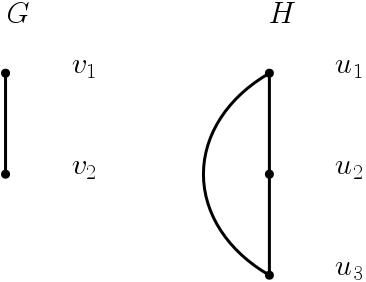
\includegraphics[scale=0.3]{GandH}
	%	\subcaption{}
	\end{minipage}
\begin{minipage}{0.45\textwidth}
	\centering
	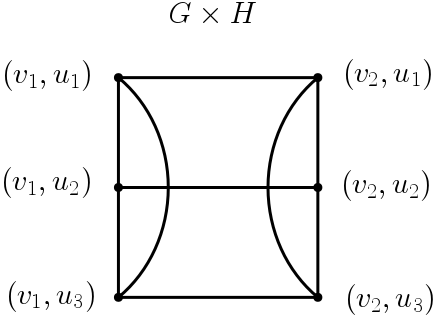
\includegraphics[scale=0.3]{GxH}
%	\subcaption{}
\end{minipage}
\caption{Two graphs and their product graph.}
\end{figure}

\begin{definition}
	\label{def:product_graphs}
	Given two graphs $G=(V(G),E(G))$ and $H=(V(H), E(H))$, the \emph{product graph of $G$ and $H$} is the graph with vertex set $V(G)\times V(H)$ and edge set
	$\{((i_1,j),(i_2,j)):(i_1,i_2)\in E(G), j\in V(H)\}\cup\{((i,j_1),(i,j_2)):(j_1,j_2)\in E(H), i\in V(G)\}$. It is denoted $G\times H$. 
\end{definition} 

In order to investigate the simplex of a product graph, we must better understand its eigenstructure. 

\begin{lemma}
	\label{lem:prod_graph_eigenstructure}
	Let graphs $G$  and $H$ be given. Put $n=|V(G)|$ and $m=|V(H)|$. Suppose $G$ has eigenvalues $\lambda_1\geq \dots\geq \lambda_{n}$ and corresponding eigenvectors $\vp_1,\dots,\vp_{n}$, as usual. Let $H$ have eigenvalues $\mu_1\geq \dots\geq \mu_{m}$ and corresponding eigenvectors $\bpsi_1,\dots,\bpsi_{m}$. Then $G\times H$ has $mn$ eigenvalues $\{\lambda_i+\mu_j\}_{(i,j)i\in[n]\times[m]}$ with eigenvectors $\{f_{i,j}\}_{(i,j)\in[n]\times[m]}$ given by 
	$f_{i,j}(k,\ell) = \vp_i(k)\bpsi_j(\ell)$. 
\end{lemma}

Consequently, with $G$ and $H$ as in Lemma~\ref{lem:prod_graph_eigenstructure}, we see that the product graph yields a simplex $\splx_{G\times H}\in\R^{mn-1}$ with vertices $\{\sv_{ij}\}_{(i,j)\in[n]\times[m]}$ given by 
\[\sv_{ij}(k\ell)=f_{k\ell}(ij)(\lambda_k+\mu_\ell)^{1/2}.\]


\subsection{Examples}
\label{sec:examples}

We now move onto concrete examples of the simplices of particular graphs whose eigenstructures we can compute explicitly. We also compute the graph of perhaps the most well-known simplex:  the probability simplex. 

\paragraph{The complete graph, $K_n$.}
Let us consider the combinatorial simplex $\splx=\splx_{K_n}$.  The Laplacian $\L_{K_n}$ has two eigenvalues: 0 with multiplicity 1 and $n$ with multiplicity $n-1$. To see this, observe that for any $\eig$ perpendicular to $\one$, we have 
\begin{align*}
\L_{K_n}\eig &= \bigg(\vp(1)(n-1)-\sum_{i\neq 1}\eg(i),\dots,\vp(n)(n-1)-\sum_{i\neq n}\eg(i)\bigg) \\
&= \bigg(\vp(1)n - \sum_i \vp(i), \dots,\vp(n)n - \sum_i \vp(i)\bigg) \\
&= (\vp(1)n,\dots,\vp(n)n) = n\eig,
\end{align*}
since $\sum_i\vp(i)=\la \eig,\one\ra =0$. Let $\Q$  described the rotation matrix which rotates each vector  by $\pi/4$  about each axis. Thus $\Q\e_1=\one$, and we can $n-1$ orthogonal eigenvectors $\Q\e_2,\dots,\Q\e_n$. The vertices of $\splx$  are thus given by $\sv_i(j) = \sqrt{n}(\Q\e_{j+1})(i)$. 

\paragraph{The Cycle graph,  $C_n$.}
The cycle graph $C_n$ has edge set $E=\{(i,j):j=i+1\mod n\}$. We assume that $n$ is even for this example. 
We leave it to the reader to verify by direct computation  that the eigenvalues  and eigenvectors of $\L_{C_n}$ are given by 
\[\vp_i(j) = \cos(\frac{2\pi(i-1)j}{n}),\quad \lambda_i = 2-2\cos(\frac{2\pi(i-1)}{n}),\]
for $i=1,\dots,n/2+1$, and 
\[\vp_i(j) = \cos(\frac{2\pi(i-n/2-1)j}{n}),\quad \lambda_i = 2-2\cos(\frac{2\pi(i-n/2-1)}{n}),\]
for $i=n/2+2,\dots,n$. Therefore,  the vertices of $\splx_{C_n}$ are given by  
\begin{equation*}
\sv_i(j) = \begin{cases}
\cos(\frac{2\pi(i-1)j}{n})\bigg(2-\cos(\frac{2\pi(i-\chi(j>n/2+1)n/2 -1)}{n})\bigg),& i\leq n/2+1, \\
\sin(\frac{2\pi(i-n/2-1)j}{n})\bigg(2-\cos(\frac{2\pi(i-\chi(j>n/2+1)n/2 -1)}{n})\bigg),& i> n/2+1.
\end{cases}
\end{equation*}


\paragraph{The probability simplex.} 
Fix  $n\in\N$. The \emph{probability simplex} is the simplex $\widetilde{\splx}_p=\conv(\{\bchi_i\}_{i=1}^n \cup \{\zero\})$. It is most likely the simplex of greatest familiarity to mathematicians and computer scientists, being used to reason geometrically about probability distributions. The probability simplex has centroid $\one/n\neq\zero$ and we will consider its centred version 
\[\splx_p \equiv \widetilde{\splx}_p -  \frac{\J}{n},\]
which has vertices  $\sv_i = \bchi_i - \one/n$, $i<n$, and $\sv_n = -\one/n$. Note that $\sv_j-\sv_n = \bchi_j$ and so 
$\la \bchi_i, \sv_j-\sv_n\ra = \delta_{ij}$. Taking  $\sv_i^\du = \bchi_i$ and $\sv_n^\du = -\sum_i \bchi_i = -\one$ thus gives us the dual vertices. The  angles between the facets of $\splx_p$ are thus defined by 
\begin{equation*}
\cos\theta_{ij}(\splx_p) = - \la \bchi_i,\bchi_j\ra = -\delta_{ij}, 
\end{equation*}
for $i,j\in[n-1]$ and 
\begin{equation*}
\cos\theta_{in}(\splx_p) = \frac{\la \bchi_i,\one\ra}{\norm{1}} = 1/\sqrt{n},
\end{equation*}
for all $i\in[n]$. 
This implies  that $\theta_{ij}(\splx_p) = 0$ for $i\neq j$, $i,j\neq n$ and $\theta_{in}(\splx_p) \in =(0,\pi/2)$. 
Using the  construction of Section~\ref{sec:simplex_to_graph}, we  associate to $\splx_p$ the graph with Laplacian matrix $\Sv(\splx_p^\du)^\to \Sv(\splx_p^\du)$, where $\Sv(\splx_p^\du)=(\sv_1^\du,\dots,\sv_n^\du)$. This matrix has $(i,j)$-th  entry $1$ for $i=j$, 1  for $i=n$ or $j=n$,  and 0 otherwise. This graph thus has each vertex connected  to $n$, but to  no others.  That  is, the graph of the probability simplex $\splx_p$ is  the star graph on  $n$ vertices. 

 



\section{Properties of \texorpdfstring{$\splx_G$}{the Combinatorial Simplex} and \texorpdfstring{$\splx_G^+$}{its inverse}}
\label{sec:S_G}
We now embark on our voyage to understand the mathematical properties of the simplices of a graph. This section is devoted to the study of $\splx_G$ and $\splx_G^+$, while Section \ref{sec:Sn_G} is concerned with $\splxn_G$ and $\splxn_G^+$. For bibliographic purposes, we will encode many of the results as Lemmas even if they are relatively simple. There are many results, and this should enable easier accounting. We begin with three basic properties.

\begin{lemma}
	\label{lem:S_G_basic_properties}
	The following three properties hold: 
	\begin{enumerate}
		\item 	Both $\splx_G$ and $\splx_G^+$ are centred at the origin;
		\item The squared distance between the vertices of $\splx_G^+$ is equal to the effective resistance between the corresponding vertices of $G$; 
		\item For any non-empty $U\subsetneq V$, the faces $\splx_U$ and $\splx^+_{U^c}$ are orthogonal. 
	\end{enumerate}
\end{lemma}
\begin{proof}
	For (i) we  simply compute $\cent(\splx) = n^{-1}\Eval^{-1/2}\Eig^\tp \one =\zero$, since $\la \vp_i,\one\ra =0$ for all $i<n$.  Likewise, $\cent(\splx^+)=\zero$. For (ii), 
	\begin{equation*}
	\norm{\sv_i^+-\sv_j^+}_2^2 = \norm{\sv_i^+}_2^2 + \norm{\sv_j^+}_2^2 - 2\la \sv_i^+,\sv_j^+\ra = \L_G^+(i,i) + \L_G^+(j,j) - 2\L_G^+(i,j) = \effr(i,j).
	\end{equation*}
	The third property follows as a result of the fact that $\splx_G^+$ is dual to $\splx_G$ (Observation \ref{obs:inverse_is_dual}) and Lemma \ref{lem:dual_faces_orthogonal}. 
\end{proof}




Property (ii) in the previous lemma was first noticed by Fielder~\cite[Chapter 6]{fiedler2011matrices}, and was also remarked upon by Van Mieghem \etal~\cite{van2017pseudoinverse} who used it in their study of best spreader nodes in electrical networks. We will return to this connection in later sections. We now turn our attention to properties of the angles of a simplex.  

\begin{lemma}
	The combinatorial simplex $\splx_G$ of a graph $G$ is hyperacute iff $\L_G^+$ is a Laplacian.
\end{lemma}
\begin{proof}
	Using Equation~\eqref{eq:cos_theta_ij} and the fact that $\splx_G^+=\splx_G^\du$ (Observation \ref{obs:inverse_is_dual}), we have
	\[\cos \theta_{ij} = -\frac{\la \sv_i^+,\sv_j^+\ra }{\norm{\sv_i^+}_2 \norm{\sv_j^+}_2},\]
	where we recall that $\theta_{ij}$ is the angle between $\splx_\ic$ and $\splx_\jc$. Thus, $\splx_G$ is hyperacute iff
	 \[-\la \sv_i^+,\sv_j^+\ra\\/\norm{\sv_i^+}_2 \norm{\sv_j^+}_2 \in[0,1],\] which occurs iff $\la \sv_i^+,\sv_j^+\ra \leq 0$. In this case $\L_G^+(i,j)\leq 0$, implying that $\L_G^+$ is a Laplacian (recall that it already satisfies the other required properties: $\L_G^+\one=\zero$ and $\L_G^+(i,i)\geq 0$). 
\end{proof}

\begin{corollary}
	\label{cor:Lkn+_laplacian}
	The combinatorial simplex of the complete graph,  $\splx_{K_n}$, is hyperacute. 
\end{corollary}
\begin{proof}
	Let $\L=\L_{K_n}$. 
	It suffices to show by the previous lemma that $\L^+=\L_{K^n}^+$ is a Laplacian. We've already seen that $\L_G^+\one=\zero$ for any $G$, so it remains only to show that $\L^+(k,k)>0$ for all $k\in[n]$ and $\L^+(k,\ell)\leq 0$ for all $k\neq\ell$, i.e., that $\sign(\L(k,\ell))=\sign(\L^+(k,\ell))$ for all $k,\ell$. Recall from Section \ref{sec:examples} that $K_n$ has eigenvalue $n$ with multiplicity $n-1$ and a single zero eigenvalue. Hence, $\L=n\sum_{i<n}\vp_i\vp_i^\tp$ and $\L^+=n^{-1}\sum_{i<n}\vp_i\vp_i^\tp$. 
	Therefore, $\sign(\L(k,\ell)) = \sign(n\sum_{i<n}\vp_i(k)\vp_i(\ell)) = \sign(\sum_{i<n}\vp_i(k)\vp_i(\ell)) = \sign(\L^+(k,\ell))$ which implies the result. 
\end{proof}


As Fiedler pointed out~\cite{fiedler1993geometric}, the correspondence also allows us to answer questions related to the distribution of angles of simplices. It is not, for example, a priori obvious that all distributions of angles  are possible in a hyperacute simplex, in the following sense. 

\begin{lemma}
	For every $n-1\leq k \leq \binom{n}{2}$, there exists a hyperacute simplex on $n$ vertices with $k$ strictly acute interior angles. 
\end{lemma}
\begin{proof}
	Fix $k$ and consider a connected graph on $n$ vertices with $k$ edges (note the importance that $k\geq n-1$). The interior angles $\{\theta_{ij}^+\}_{i,j}$ of $\splx_G^+$ obey $\cos\theta_{ij} = w(i,j) / \sqrt{w(i)w(j)}$, hence $\theta_{ij}=\pi/2$ whenever $w(i,j)=0$, and $\theta_{ij}\in(0,\pi/2)$ for all $(i,j)\in E(G)$. Therefore, $\splx_G^+$ meets the desired criteria. 
\end{proof}



The following lemma presents an alternate characterization of the simplex, and was first proved by Devriendt  and Van Mieghem~\cite{devriendt2018simplex}. As they notice, the following representation provides an easy way to check whether a given point lies inside the simplex. As our proof is similar  to theirs, we move  it to  Appendix~\ref{sec:app_proofs_correspondence}. 

\begin{lemma}[\cite{devriendt2018simplex}]
\label{lem:S_alt_desc}
For a simplex $\splx$ of a graph $G$, 
\begin{equation}
\label{eq:S_alt_desc}
    \splx=\bigg\{\x\in \R^{n-1}:\x^\tp\Sv^++\frac{\one^\tp}{n}\geq \zero^\tp\bigg\}.
\end{equation}
\end{lemma}

Just as each facet of a tetrahedron is contained in a plane and each edge is contained in an infinite line, each face $\splx_U$ of a simplex $U$ is contained in a \emph{flat} \note{Need to define  this} of dimension $|U|-1$. The following lemma helps characterize these flats. 

\begin{lemma}
\label{lem:SUsubset}
Let $\splx$ be the simplex of a graph $G=(V,E,w)$, and fix $U\subset V$. For any non-empty $E\subset U^c$,
\begin{equation*}
    \splx_U \subset \bigg\{\x\in\R^{n-1}: \sum_{i\in E}\la \x,\sv_i^+\ra +\frac{|E|}{n}=  0\bigg\},
\end{equation*}
and
\begin{equation*}
    \splx^+_U \subset \bigg\{\x\in\R^{n-1}: \sum_{i\in E}\la \x,\sv_i\ra +\frac{|E|}{n}=  0\bigg\},
\end{equation*}
\end{lemma}
\begin{proof}
Let $\x\in\splx_U$ be arbitrary. For any $i\in U^c$ we have $\la \x,\sv_i^+\ra = -1/n$. Hence, for any $E\subset U^c$
\[\sum_{i\in E}\la \x,\sv_i^+\ra + \frac{|E|}{n} = \sum_{i\in E}\bigg(\la \x,\sv_i^+\ra+\frac{1}{n}\bigg)=\sum_{i\in E}\bigg(\frac{1}{n}-\frac{1}{n}\bigg)=0,\]
implying that $\x$ is in the desired set. 
\end{proof}

Lemma \ref{lem:SUsubset} gives us an alternate way to prove Lemma \ref{lem:S_alt_desc}. For any $i$,  taking $U=N\setminus \{i\}$ and $E=\{i\}$, it implies that $\splx_{\{i\}^c}$ is a subset of the hyperplane 
\begin{equation}
\label{eq:Hi}
 \H_i\equiv \{\x\in\R^{n-1}:\la \x,\sv_i^+\ra+1/n=0\}.
\end{equation}
All points in the simplex $\splx$ lie to one side of $\splx_{\{i\}^c}$, i.e., they lie in the halfspace 
\[\H_i^{\geq } \equiv \{\x\in\R^{n-1}:\la \x,\sv_i^+\ra+1/n\geq0\}.\]
(We know it is this halfspace because $\zero\in\splx\cap\H_i^{\geq }$.) The simplex is the interior of the region defined by the intersection of the faces $\splx_{\{i\}^c}$, i.e.,   
\begin{equation}
\label{eq:splx_bigcapH_i}
    \splx=\bigcap_i \H_i^{\geq }.
\end{equation}
Moreover, $\x\in \bigcap_i\H_i^{\geq }$ iff $\la \x,\sv_i^+\ra +1/n\geq 0$ for all $i$, i.e., $(\la \x,\sv_1^+\ra,\dots,\la \x,\sv_n^+\ra) + \one/n\geq \zero$, meaning $\x$ satisfies \eqref{eq:S_alt_desc}.  We emphasize that a very similar discussion applies to $\splx^+$, in which case one has 
\begin{equation}
\label{eq:splx^+_bigcapH_i}
\splx^+=\bigcap_i (\H_i^+)^{\geq },
\end{equation}
for $(\H_i^+)^{\geq } \equiv \{\x\in\R^{n-1}:\la \x,\sv_i\ra + 1/n\geq 0\}$. 

\begin{figure}
	\centering
	\includegraphics[scale=0.5]{HI_plane}
	\caption{An illustration of the combinatorial simplex $\splx_G\subset\R^3$ and its face $\splx_\ic$ contained in the hyperplane $\H_i$. }
	\label{fig:Hi_plane}
\end{figure}


\paragraph{Centroids and altitudes.} 
We now turn to investigating the centroids and altitudes of the simplices, and how they relate to properties of the underlying graph. We begin by exploring the relationships between properties of the simplices themselves. 

Recall that the altitude between $\splx[U]$ and $\splx[U^c]$ of a simplex $\splx$ is denoted $\alt(\splx_U)$ and is the unique vector $\p-\q$ where  $\p\in \splx_{U^c}$ and $\q\in\splx_{U}$ which lies in the orthogonal complement of both $\splx_U$ and $\splx_{U^c}$. One would thus expect that $\alt(\splx_U)$ and $\alt(\splx_{U^c})$ to be antiparallel; a fact verified by Lemma \ref{lem:complimentary_centroids}.  

In what follows,  we will often write $\cent_U$ for $\cent(\splx_U)$ (resp., $\cent_U^+$ for $\cent(\splx_U^+)$) and $\alt_U$ for $\alt(\splx_U)$ (resp., $\alt_U^+$ for $\alt(\splx_U^+)$). 

\begin{lemma}[\cite{devriendt2018simplex}]
\label{lem:complimentary_centroids}
Let $U\subset V$ be non-empty. Then the vectors $\cent(\splx_U)$ and $\cent(\splx_{U^c})$ are antiparallel. In particular, $(n-|U|)\cent(\splx_{U^c}) = |U|\cent(\splx_{U})$ and 
\[\frac{\cent(\splx_U)}{\norm{\cent(\splx_U)}_2}=-\frac{\cent(\splx_{U^c})}{\norm{\cent(\splx_{U^c})}_2}.\]
\end{lemma}
\begin{proof}
This is a straightforward computation: Observing that $\bchi_U=\one-\bchi_{U^c}$ we have  
\[\cent_U = |U|^{-1}\Sv\bchi_U = |U|^{-1}\Sv(\one-\bchi_{U^c})=-|U|^{-1}\Sv\bchi_{U^c}=-|U|^{-1}\frac{|U^c|}{|U^c|}\Sv\bchi_{U^c}=\frac{n-|U|}{|U|}\cent_{U^c},\]
where we've used that $\Sv\one=\zero$. This proves the first result; the second follows from normalizing the two vectors.
\end{proof}

We would now like to examine the relationships between altitudes and centroids in the simplex and its inverse. We will demonstrate that centroids of opposing faces are antiparallel, and that the centroid of the face $U$ is parallel to the altitude of originating from the face generated by $U$ in its inverse. First however, we require the following technical result. 

\begin{lemma}
	\label{lem:S_U_ortho_complement}
	Any vector perpendicular to $\splx_U$ can be written as $\Sv^+(\f_{U^c}+\alpha \bchi_U)$ for some $\alpha\in\R$ and vector $\f_{U^c}$ such that $\f_{U^c}(U)=\zero$. 
\end{lemma}
\begin{proof}
	Let $\y\in\R^{n-1}$ be orthogonal to $\splx_U$. Since $\rank(\Sv^+)=n-1$, we can find some $\z$ such that $\y=\Sv^+\z=\sum_{i\in U^c}\sv_i^+z(i) + \sum_{j\in U}\sv_j^+z(j)$. Define $\f$ by $\f(U^c)=\z(U^c)$ and $\f(U)=\zero$ and $\z_{U^c}$.  We can then write $\y$ as $\Sv^+\f+\sum_{j\in U}\sv_j^+z(j)$, so we must show that $\z(U)$ is a constant vector. The orthogonality of $\y$ to $\splx_U$ implies that for every two barycentric coordinates $\x_U$ and $\y_U$ with $\x(U^c)=\y(U^c)=\zero$, 
	\begin{align}
	0 &= \la \y,\Sv\x_U-\Sv\y_u\ra \notag \\
	&= \sum_{i\in U^c}z(i) \la \sv_i^+,\Sv(\x_U-\y_U)\ra + \sum_{j\in U}z(j)\la \sv_j^+,\Sv(\x_U-\y_U)\ra  \notag \\
	&= \sum_{j\in U}z(j)\la \sv_j^+,\Sv(\x_U-\y_U)\ra, \label{eq:lem_ortho_complement1}
	\end{align} 
	where the final inequality follows because $\sv_i^+$ is orthogonal to $\splx_U$ for $i\in U^c$ by Lemma \ref{lem:S_G_basic_properties}.
	 Now, for $j\in U$, 
	\begin{align}
	\la \sv_j^+,\Sv(\x_U-\y_U)\ra &= \bchi_j^\tp \Sv^+\Sv(\x_U-\y_U) = \bchi_j^\tp \bigg(\I - \frac{\J}{n}\bigg)(\x_U-\y_U) = \bchi_j^\tp (\x_U-\y_U). \label{eq:lem_ortho_complement2}
	\end{align}
	Suppose for contradiction that $z(k)\neq z(j)$ for some $k,j\in U$. Put $\x_U = \bchi_k$ and $\y_U=\bchi_j$. Using Equation  \eqref{eq:lem_ortho_complement2} write \eqref{eq:lem_ortho_complement1} as 
	\begin{align*}
	z(k)\bchi_k^\tp(\bchi_k-\bchi_j) + z(j)\bchi_j^\tp(\bchi_k -\bchi_j) + \sum_{\ell\in U^c,\ell\neq j,k}z(\ell)\bchi_\ell^\tp(\bchi_k-\bchi_j) = z(k)-z(j)\neq 0,
	\end{align*}
	a contradiction. 
\end{proof}

We can now proceed to the main result. 

\begin{lemma}
\label{lem:alt_and_centroid}
For a simplex $\splx$ of a graph $G=(V,E)$ and any $U\subset V$, $U\neq\emptyset$, 
\begin{equation}
\label{eq:alt_and_centroid}
    \frac{\alt(\splx_U)}{\norm{\alt(\splx_{U})}_2}=\frac{\cent^+(\splx_{U^c})}{\norm{\cent^+(\splx_{U^c})}_2}=-\frac{\cent^+(\splx_{U})}{\norm{\cent^+(\splx_{U})}_2},
\end{equation}
and 
\begin{equation*}
    \frac{\alt^+(\splx_U)}{\norm{\alt^+(\splx_{U})}_2}=\frac{\cent(\splx_{U^c})}{\norm{\cent(\splx_{U^c})}_2}=-\frac{\cent(\splx_{U})}{\norm{\cent(\splx_{U})}_2}.
\end{equation*}
\end{lemma}
\begin{proof}
We prove the first set of equalities only; the second is obtained similarly. By definition, $\alt_U$ is orthogonal to both $\splx_U$ and $\splx_{U^c}$. Lemma \ref{lem:S_U_ortho_complement} then implies both that 
\begin{equation*}
\alt_U = \Sv^+\f + \alpha \Sv^+\bchi_U,
\end{equation*}
and 
\begin{equation*}
\alt_U = \Sv^+\g + \beta\Sv^+\bchi_{U^c},
\end{equation*}
for some $\alpha,\beta\in\R$, and vectors $\f,\g$ with $\f(U)=\zero$ and $\g(U^c)=\zero$. In particular then, 
\begin{equation}
\label{eq:lem_alt_centroid1}
\frac{\Sv^+(\f+\alpha\bchi_U)}{\norm{\Sv^+(\f+\alpha\bchi_U)}_2}=\frac{\Sv^+(\g+\beta\bchi_{U^c})}{\norm{\Sv^+(\g+\beta\bchi_{U^c})}_2}.
\end{equation}
By Lemma \ref{lem:complimentary_centroids}, taking $\f=\pm\bchi_{U^c}/|U^c|$, $\g=\mp\bchi_U/|U|$, and $\alpha=\beta=0$ yield solutions to the above equation. We have thus obtained Equation \eqref{eq:alt_and_centroid} up to its sign; 
it remains to determine whether $\alt(\splx_U)$ is parallel to antiparallel to $\cent(\splx_U)$. Since it is one of the two, we have 
\[\frac{\la \alt_U,\cent^+_U\ra}{\norm{\alt_U}_2\norm{\cent^+U}_2}\in\{1,-1\},\]
hence to see that they are antiparallel it suffices to show that $\la \alt_U,\cent^+U\ra<0$. Let $\alt_U= \Sv\y_{U^c}-\Sv\z_U$ for barycentric coordinates $\y_{U^c}$ and $\z_U$ representing the faces $\splx_{U^c}$ and $\splx_U$. Then, 
\begin{align*}
\la \alt_U,\cent^+_U\ra &= \frac{1}{n}\la \Sv(\y_{U^c}-\z_U),\Sv\bchi^+_U\ra \\
&= \frac{1}{n}(\y_{U^c}^\tp-\z_U^\tp)\bigg(\I-\frac{\J}{n}\bigg)\bchi_U\\ &=-\frac{1}{n}\z_U^\tp\bchi_U  - \frac{1}{n^2}(\y_{U^c}^\tp-\z_U^\tp)\one\one^\tp\bchi_U\\
&= -\frac{1}{n}<0.
\end{align*}
Therefore, $\alt_U$ is indeed antiparallel to $\cent^+_U$, meaning that the correct signage is $\f=\bchi_{U^c}/|U^c|$ and $\g=-\bchi_U/|U|$. Thus, 
\begin{equation*}
\frac{\alt_U}{\norm{\alt_U}_2}=\frac{\Sv^+\bchi_{U^c}}{\norm{ \Sv^+\bchi_{U^c}}_2}=-\frac{\Sv^+\bchi_{U}}{\norm{\Sv^+\bchi_U}_2},
\end{equation*}
which is Equation \eqref{eq:alt_and_centroid}. 
\end{proof}

\begin{remark}
	We note that there are no other solutions, up to scaling, of the system of equations for $\alt_U$ in the previous proof. Indeed, let $\f,\g,\alpha,\beta$ satisfy the equations. 
	Then 
	\[\Sv^+(\f-\beta\bchi_{U^c}) + \Sv^+(\alpha\bchi_U-\g)=\zero, \]
	so $f-\beta\bchi_{U^c} + \alpha\bchi -g\in \ker(\Sv^+) = \spn(\one)$, implying that $\f-\beta\bchi_{U^c} = k\bchi_{U^c}$ and $\alpha\bchi_U -g=k\bchi_{U}$ for some $k\in \R$, which yields the same solution as in the proof. 
\end{remark}

Whereas the previous few lemmas explored relationships among $\splx_G$ and $\splx_G^+$ only, we now begin to observe several connections between the geometry of the simplices and properties of the graph. We begin by recalling that given $U\subset V(G)$ the \emph{cut-set} of $U$ is 
\[\partial U \equiv (U\times U^c)\cap E(G)= \{(i,j)\in E(G): i\in U, j\in U^c\}.\]
Noting that $|\bchi_U(i)-\bchi_U(j)|=\chi_{(i,j)\in \partial U}$, we see that
\begin{align*}
w(\partial U) = \sum_{i,j\in E} w(i,j)|\bchi_U(i)-\bchi_U(j)| = \sum_{i,j\in E} w(i,j)(\bchi_U(i)-\bchi_U(j))^2 = \Lf(\bchi_U). 
\end{align*}
Moreover, $\norm{\cent(\splx_U)}^2_2 = \la |U|^{-1} \Sv\bchi_U,|U|^{-1} \Sv\bchi_U\ra = |U|^{-2} \Lf(\bchi_U)$ and so 
\begin{equation}
\label{eq:c(S_U)}
\norm{\cent(\splx_U)}_2^2 = \frac{w(\partial U)}{|U|^2}.
\end{equation}
Via the same process we can also obtain an equivalent expression for the centroid of the inverse simplex: 
\begin{equation}
\label{eq:c(S+_U)}
\norm{\cent(\splx^+_U)}_2^2 = \frac{w(\partial^+ U)}{|U|^2},
\end{equation}
where we follow the notation of \cite{devriendt2018simplex} and define \begin{equation}
\label{eq:w(d^+)}
w(\partial^+U) \equiv  \la \Sv^+\bchi_U,\Sv^+\bchi_U\ra=\la \bchi_U,\L^+\bchi_U\ra=\Lf^+(\bchi_U).
\end{equation} 
Equations \eqref{eq:c(S_U)} and \eqref{eq:c(S+_U)} were also given in \cite{devriendt2018simplex}. As a sanity check, we note that the equations are consistent with the facts that $\norm{\sv_i}_2^2 = w(i)$ and $\norm{\sv_i^+}_2^2 = \L^+(i,i) = \Lnf^+(\bchi_i)$. These equations allow us to give an interesting correspondence between the sizes of the altitudes and cut-sets of $G$. 

\begin{lemma}
\label{lem:||alt||}
For any non-empty $U\subset V$, $\norm{\alt^+_U}_2^2=1/w(\partial U)$ and $\norm{\alt_U}_2^2 = 1/w(\partial^+ U)$.  
\end{lemma}
\begin{proof}
By definition of the altitude there exists barycentric coordinates $\x_U$ and $\x_{U^c}$ such that $\alt^+_U = \Sv^+(\x_U-\x_{U^c})$. Combining this representation of $\alt^+_U$ with that given by Lemma \ref{lem:alt_and_centroid}, write 
\begin{align*}
    \norm{a^+_U}_2 = \frac{\la a^+_U,a^+_U\ra }{\norm{a^+_U}_2} = \frac{\la \Sv^+(\x_{U^c}-\x_{U}), c_{U^c}\ra }{\norm{c_{U^c}}_2} = \frac{\la \Sv^+(\x_{U^c}-\x_{U}), \Sv\bchi_{U^c}\ra }{\sqrt{w(\partial U^c)}},
\end{align*}
where the final equality comes from using the definition of the centroid in the numerator, and Equation~\eqref{eq:c(S_U)} in the denominator. Recalling the relation between $\Sv$ and $\Sv^+$ given by Equation~\eqref{eq:sv+sv} and that $\x_U$ and $\x_{U^c}$ are barycentric coordinates, we can rewrite the above as 
\[\frac{(\x_{U^c}-\x_{U})^\tp(\I-\one\one^\tp/n)\bchi_{U^c}}{\sqrt{w(\partial U^c)}}=\frac{1}{\sqrt{w(\partial U^c)}}. \]
Squaring both sides while noting that $\partial U = \partial U^c$ completes the proof of the first equality. For the second, we proceed in precisely the same manner to obtain $\norm{a_U}_2^2 = 1/w(\partial^+ U^c)$. However, it's not immediately obvious that $w(\partial^+U^c)=w(\partial^+U)$. To see this, first recall that $\Sv^+\one = \Eval^{-1/2}\Eig^\tp\one = \zero$, and so 
\begin{align*}
w(\partial^+ U^c) &= \la \Sv^+\bchi_{U^c},\Sv^+\bchi_{U^c}\ra  \\
&= \la \Sv^+(\one - \bchi_{U}),\Sv^+(\one - \bchi_{U})\ra  \\
&= \la \Sv^+\bchi_{U},\Sv^+\bchi_{U}\ra = w(\partial^+ U).
\qedhere
\end{align*}
\end{proof}

The aforementioned astute reader may have noticed that the above result implies something about the computational difficulty of determining the length of the minimum and maximum altitudes in hyperacute simplices. We tell this reader to ``hold their horses''---this result and others like it will be presented in Chapter \ref{chap:algorithmics}. 

The next two lemmas were both proven by Devriendt and Van Mieghem~\cite{devriendt2018simplex}, extending work done by Fiedler. 
The following lemma gives an explicit expression for the altitudes in terms of graph properties and the inverse centroid. 

\begin{lemma}
\label{lem:alt}
For any non-empty $U\subset V$, 
\[\alt_U=\frac{n-|U|}{w(\partial^+ U)}\cent^+_{U^c},\quad \text{and}\quad \alt^+_U = \frac{n-|U|}{w(\partial U)} \cent_{U^c}.\]
\end{lemma}
\begin{proof}
This is a consequence of identities \eqref{eq:c(S_U)} and \eqref{eq:c(S+_U)} and Lemmas \ref{lem:alt_and_centroid} and \ref{lem:||alt||}. Applying the latter and then the former, observe that 
	\[\alt_U = \frac{\norm{\alt_U}_2}{\norm{\cent^+_{U^c}}_2}\cent^+_{U^c} =
\bigg(\frac{1}{\sqrt{w(\partial^+ U^c)}} \bigg/\frac{\sqrt{w(\partial^+U)}}{|U^c|} \bigg)\cent^+_{U^c} = \frac{n-|U|}{w(\partial^+U)}c^+_{U^c},\]
where we've once against used that $w(\partial^+ U^c )=w(\partial^+ U)$. A similar computation holds for $\alt_U^+$.  
\end{proof}

Just as one generalizes the incidence of a vertex to the neighbourhood of a set of vertices, one can generalize an edge to the incidence between groups of vertices, as
\[\partial U_1\cap \partial U_2 = \{(i,j)\in E(G), i\in U_1,j\in U_2\},\]
for $U_1,U_2\subset V(G)$. The final lemma gives an expression for the weight (or size) of this set in terms of the altitudes and centroids of the simplices. 


\begin{lemma}
	\label{lem:alt_centroid_dot_product}
Let $U_1,U_2\subset V$ with $U_1\cap U_2=\emptyset$. Then 
\begin{equation*}
    \la \cent(\splx_{U_1}),\cent(\splx_{U_2})\ra = - \frac{w(\partial U_1\cap \partial U_2)}{|U_1||U_2|},\quad\text{and}\quad \la \alt^+_{U_1},\alt^+_{U_2}\ra = -\frac{w(\partial U_1^c\cap \partial U_2^c)}{w(\partial U_1)w(\partial U_2)}.
\end{equation*}
\end{lemma}
\begin{proof}
For $i,j\in V$, $i\sim j$, observe that 
\[\bchi_{U_1}^\tp \L_{i,j}\bchi_{U_2}=
\begin{cases}
-w(i,j),& i\in U_1,j\in U_2\text{ or }i\in U_2,j\in U_1,\\
0,&\text{otherwise.}
\end{cases}\]
Therefore, 
\begin{align*}
    \la \cent_{U_1},\cent_{U_2}\ra &= \la |U_1|^{-1}\Sv\bchi_{U_1},|U_2|^{-1}\Sv\bchi_{U_2}\ra = |U_1|^{-1}|U_2|^{-1} \bchi_{U_1}^\tp \L_G\bchi_{U_2} \\
    &= |U_1|^{-1}|U_2|^{-1}\sum_{i\sim j} \bchi_{U_1}^\tp \L_{(i,j)}\bchi_{U_2} = |U_1|^{-1}|U_2|^{-1}\sum_{(i,j)\in \partial U_1\cap \partial U_2} -w(i,j),
\end{align*}
which proves the first equality. The second is shown similarly by employing Lemma \ref{lem:alt} and the previous identity:
\begin{align*}
    \la \alt^+_{U_1},\alt^+_{U_2}\ra &= \frac{|U_1^c||U_2^c|}{w(\partial U_1) w(\partial U_2)}\la \cent_{U_1^c},\cent_{U_2^c}\ra
    =-\frac{w(\partial U_1^c\cap \partial U_2^c)}{w(\partial U_1)w(\partial U_2)}.\qedhere
\end{align*}
\end{proof}

Given the number of---often related and interacting---results in this section, it may be worth providing a brief summary. The important takeaways are that (i) the geometry of the inverse simplex $\splx^+$ is intimately related to the effective resistance of the graph (Lemma \ref{lem:S_G_basic_properties}) and (ii) the lengths of the altitudes and centroids of $\splx$ and $\splx^+$ are proportional to the weights of cuts (Equations \eqref{eq:c(S_U)}, \eqref{eq:c(S+_U)}, Lemmas \ref{lem:||alt||}, \ref{lem:alt}, \ref{lem:alt_centroid_dot_product}). 

\section{Properties of \texorpdfstring{$\splxn_G$}{the normalized Simplex} and \texorpdfstring{$\splxn_G^+$}{and its inverse}}
\label{sec:Sn_G}

Here we study the normalized simplex $\splxn_G$ of the connected graph $G=(V,E,w)$---which we again fix throughout this section---a somewhat less accessible object than its unnormalized counterpart.  The normalized simplex is, roughly speaking, distorted by the weights of the vertices. Consequently, many of the relationships between $\splx_G$ and $\splx_G^+$ are lost between $\splxn_G$ and $\splxn_G^+$. The first issue is that, in general, $\splxn_G$ and its inverse are not centred at the origin. Indeed, recall that the zero eigenvector $\vpn_n$ of $\Ln_G$ sits in the space $\spn(\W^{1/2}_G\one)$, which is distinct from $\spn(\one)$ unless $\W^{1/2}_G=d\I$ for some $d$, in which case $G$ is regular.
If $G$ is not regular, we thus have that $\vp_i \in \spn(\W^{1/2}_G\one)\subset \spn(\one)^\perp$ for all $i<n$ implying that $\la \vp_i,\one\ra \neq 0$. In this case then,  
 \[\cent(\splxn_G) = \frac{1}{n} \Evaln^{1/2}\Eign^\tp \one = \frac{1}{n} \begin{pmatrix}
 \sqrt{\lambda_1}\la \vp_1,\one\ra \\
 \vdots \\
\sqrt{ \lambda_{n-1}}\la \vp_{n-1},\one \ra
 \end{pmatrix}\neq \zero.\]
The above argument proves the following.

\begin{lemma}
	\label{lem:centroid_normalized}
	The centroid of $\splxn_G$ coincides with the origin of $\R^{n-1}$ iff $G$ is regular. 
\end{lemma}

Given this, one might wonder whether the origin is even a point in the simplex $\splxn$. It is easily seen that it is, however. Consider the barycentric coordinate $\u = \sqrt{\w}/\norm{\sqrt{\w}}_1$, where $\sqrt{\w}=(w(1)^{1/2}, \dots, w(n)^{1/2})$. Since all eigenvectors $\vpn_i$, $i<n$ are orthogonal to $\vp_n \in\spn(\w^{1/2})$ it follows that $\zero = \Svn\u\in\splxn$. 

The next set of properties which don't hold between $\splxn$ and $\splxn^+$ are the orthogonality relationships present between a simplex and its dual. That is, in general $\splxn^+_G$ is the not the dual of $\splxn_G$. 

\begin{lemma}
	\label{lem:inverse_not_dual}
	The inverse simplex $\splxn_G^+$ is the dual of $\splxn_G$ iff $G$ is regular. 
\end{lemma}
\begin{proof}
	For any $i,j,k\in\N$ write 
	\begin{equation}
	\label{eq:lem_inverse_not_dual}
	\la \svn_i^+,\svn_j-\svn_k\ra = \delta_{ij} - \delta_{ik} + \frac{\sqrt{w(i)w(k)}}{n} - \frac{\sqrt{w(i)w(j)}}{n}.
	\end{equation}
	First suppose that $G$ is regular; so  $w(r)=w(s)$ for all $r,s$. Then for $i\neq k$, Equation \eqref{eq:lem_inverse_not_dual} becomes $\la \svn_i^+,\svn_j-\svn_k\ra = \delta_{ij}$. Since $k$ was arbitrary, we see that $\{\svn_i^+\}$ is the sister pair of $\{\svn_j-\svn_k\}$. Conversely, suppose $G$ is not regular and let $i,k$ obey $0\neq w(i)\neq w(k)$. Taking $i=j\neq k$ in \eqref{eq:lem_inverse_not_dual} we see 
	\[\la \svn_i^+,\svn_i-\svn_k\ra = 1 - \frac{\sqrt{w(i)}}{n}(\sqrt{w(k)}-\sqrt{w(i)})\neq 1,\]
	so $\{\svn_i^+\}$ is not the sister set of $\{\svn_j-\svn_k\}$, completing the argument. 
\end{proof}

A consequence of the previous Lemma is that we can no longer apply Lemma \ref{lem:dual_faces_orthogonal} (regarding the orthogonality of $\ssplx_U$ and $\ssplx_{U^c}^\du$) to obtain information concerning $\splxn_U$ and $\splxn_{U^c}^+$. The following two lemmas and corresponding corollary address the link between these faces, and---rather unfortunately---demonstrate that indeed, they are not orthogonal in general. 
The first gives sufficient conditions under which the faces are orthogonal, the second provides necessary conditions. 
Before we state the lemmas, recall from Section \ref{sec:background_spectral} that a subset of vertices is weight  (or degree) homogenous if each vertex in the set has the same weight. 

\begin{lemma}
	\label{lem:Sn_perp_homogenous}
	Let $U_1,U_2\subset V(G)$ be two non-empty, weight homogenous subsets such that $U_1\cap U_2=\emptyset$. Then the faces $\splxn^+[U_1]$ and $\splxn[U_2]$ are orthogonal. 
\end{lemma}
\begin{proof}
	Suppose $w(i)=w_1$ for all $i\in U_1$ and $w(i)=w_2$ for all $i\in U_2$. Let $\x_{U_1}$ be the barycentric coordinate of any point in $\splxn^+[U_1]$ and $\x_{U_2}$ that of any point in $\splxn[U_2]$. 
	\begin{align*}
	\la \Svn^+\x_{U_1},\Svn\x_{U_2}\ra &= \x_{U_1}^\tp \bigg(\I-\frac{\sqrt{\w}\sqrt{\w}^\tp}{\vol(G)}\bigg) \x_{U_2}\\
	&= \x_{U_1}^\tp\x_{U_2} - \frac{1}{\vol(G)}\sum_{i\in U_1}\x_{U_1}(i)\sqrt{w(i)}\sum_{j\in U_2}\x_{U_2}(j) \sqrt{w(j)} \\
	&= -\frac{1}{\vol(G)}\sqrt{w_1w_2}\sum_{i\in U_1}\x_{U_1}(i) \sum_{j\in U_2}\x_{U_2}(j) = -\frac{\sqrt{w_1w_2}}{\vol(G)},
	\end{align*} 
	where the second equality is due to fact that $U_1\cap U_2=\emptyset$. This demonstrates that $\la \Svn^+\x_{U_1},\p-\q\ra=0$ for any $\p,\q\in\splxn[U_2]$, completing the proof. 
\end{proof}

\begin{lemma}
	\label{lem:Sn_not_homogeneous}
	Suppose  $U_1\subset V(G)$ is not degree homogeneous. Then for all $U_2\subset V(G)$ then faces $\splxn[U_1]$ (resp., $\splxn^+[U_1]$) and $\splxn^+[U_2]$ (resp., $\splxn[U_2]$) are not orthogonal. 
\end{lemma}
\begin{proof}
	We show that $\splxn[U_1]$ and $\splxn^+[U_2]$ are not orthogonal; the other case is nearly identical. Let $i,j\in U_1$ be such that $w(i)\neq w(j)$ and consider the points $\p=\Svn\bchi_i,\q=\Svn\bchi_j\in\splxn[U_1]$. For any $\Svn^+\x\in\splxn^+[U_2]$, performing the usual arithmetic yields
	\begin{align*}
	\la \Svn^+\x,\p-\q\ra &= \frac{1}{\vol(G)} \sum_{k\in U_2}\sqrt{w(k)}x(k)(\sqrt{w(j)}-\sqrt{w(j)}) \neq 0.\qedhere
	\end{align*}
\end{proof}

We state a consequence of Lemmas \ref{lem:Sn_perp_homogenous} and \ref{lem:Sn_not_homogeneous} which exemplifies a clear contrast between  the combinatorial simplices and the normalized simplices.   

\begin{corollary}
	\label{cor:Sn_orthog_iff_regular}
	The vertex $\svn_i^+$ (resp., $\svn_i$) is orthogonal to $\splxn_\ic$ (resp., $\splxn^+_\ic$) iff $G[\ic]=G[V\setminus\{i\}]$ is regular. 
\end{corollary}
\begin{proof}
	If $G[\ic]$ is regular then $\ic$ is weight homogenous. By Lemma~\ref{lem:Sn_perp_homogenous} $\splxn[\{i\}]=\svn_i$ (resp., $\splxn^+[\{i\}]=\svn_i^+$) is orthogonal to $\splxn[\ic]$ (resp., $\splxn^+[\ic]$). (Note that the singleton $\{i\}$ is clearly degree homogeneous.) Conversely, if $G[\ic]$ is not regular then by Lemma~\ref{lem:Sn_not_homogeneous} $\svn_i$ (resp., $\svn_i^+$) is not orthogonal to $\splxn[\ic]$ (resp., $\splxn^+[\ic]$).
\end{proof}

\paragraph{Centroids and altitudes.}
Let us attempt to parallel the arguments given in Section~\ref{sec:S_G}  concerning the centroids and altitudes of $\splx_G$ and $\splx_G^+$. For the normalized Laplacian we have
\begin{align}
\Lnf(\bchi_U)&=\sum_{i\sim j}w(i,j) \bigg(\frac{\bchi_U(i)}{\sqrt{w(i)}}-\frac{\bchi_U(j)}{\sqrt{w(j)}}\bigg)^2 \notag \\
&= \sum_{i\in U,j\in U^c}w(i,j)\bigg(\frac{\bchi_U(i)}{\sqrt{w(i)}}-\frac{\bchi_U(j)}{\sqrt{w(j)}}\bigg)^2 \notag \\
&= \sum_{i\in U,j\in U^c}w(i,j)\frac{\bchi_U(i)}{w(i)} \notag \\
&= \sum_{i\in U}\frac{1}{w(i)} \sum_{j\in \partial(i)\cap U^c}w(i,j) \notag \\
&= \sum_{i\in U}\frac{w_{G[i+U^c]}(i)}{w(i)}, \label{eq:Lnf(chiU)}
\end{align}
where we've used the shorthand $i+U^c = \{i\}\cup U^c$ and we recall that $G[I]$ is the graph restricted to the vertices in $I$. 
To interpret the above quantity, we might define  
\[\gamma(i,B)\equiv \frac{w_{G[i+B^c]}(i)}{w(i)},\]
as the \emph{fractional weight of $i$ in $B$}. 
Further defining $\gamma(A,B)$ as the \emph{total fractional weight from $A$ to $B$}:
\[\gamma(A,B) \equiv \sum_{i\in A}\gamma(i,B), \]
we have 
$\Lnf(\bchi_U) = \gamma(U,U^c)$, 
and so the length of the centroid $c(\splxn_U)$ captures the total fraction of weight between $U$ and $U^c$:
\begin{equation}
\label{eq:c(SnU)}
\norm{c(\splxn_U)}_2^2 = \frac{1}{|U|^2}\la \Svn\chi_U,\Svn\chi_U\ra = \frac{1}{|U|^2}\Lnf(\chi_U) = \frac{1}{|U|^2} \gamma(U,U^c),
\end{equation}
which is the equivalent to Equation \ref{eq:c(S_U)} for the normalized simplex. Performing a similar computation for $\cent(\splxn^+_U)$ doesn't seem to yield anything overly insightful. 


\paragraph{Alternate descriptions and duals.} As we did for the combinatorial simplices, we now try to formulate a hyperplane representation of the normalized simplices. As the reader will see, however, this is difficult due to the influence of the graph weights on their geometry. We begin with a lemma which is roughly the equivalent of Lemma \ref{lem:SUsubset} for the normalized simplex. 

\begin{lemma}
	\label{lem:SUn_subset}
	Let $U\subset V$ be non-empty and $F\subset U^c$. Setting 
	\[\beta_i^S = \sqrt{w(i)} \frac{\max_{j\in S} \sqrt{w(j)}}{\vol(G)},\]
	for any set $S$, we have 
	\begin{equation*}
	\splxn_U \subset \Hn_{F}^\geq \equiv \bigg\{\x\in\R^{n-1}: \sum_{i\in F} (\la \x,\svn_i^+\ra + \beta_i^{F^c})\ge 0\bigg\}.
	\end{equation*}
	Similarly, 
	\begin{equation*}
	\splxn^+_U \subset (\Hn^+_{F})^\geq \equiv \bigg\{\x\in\R^{n-1}: \sum_{i\in F} (\la \x,\svn_i\ra + \beta_i^{F^c})\ge 0\bigg\}.
	\end{equation*}
\end{lemma} 
\begin{proof}
	Let $\x=\Svn\y\in \splxn_U$, where $\y$  is a barycentric coordinate with $\y(U^c)=\zero$. For $i\in U^c$, 
	\begin{align*}
	\la \Svn\y,\svn_i^+ \ra &= \y^\tp \Svn^\tp \Svn^+ \bchi_i = \y^\tp \bigg(\I-\frac{\sqrt{\w}\sqrt{\w}^\tp}{\vol(G)}\bigg)\bchi_i = - \frac{1}{\vol(G)} \left(\sum_{j\in U}y(j) \sqrt{w(j)}\right) \sqrt{w(i)}.
	\end{align*}
	Since $\norm{\y}_1=1$, and $F^c\supset U$ (since $F\subset U^c$) it follows that 
	\[\sum_{j\in U}y(i) \sqrt{w(j)} \leq \max_{j\in U} \sqrt{w(j)} \leq \max_{j\in F^c}\sqrt{w(j)},\]
	hence 
	\[\la \Svn\y,\svn_i^+\ra \geq -\frac{\sqrt{w(i)}}{\vol(G)} \max_{j\in F^c}\sqrt{\w(j)} = -\beta_i^{F^c}.\]  
	Consequently, $\sum_{i\in F} (\la \x,\svn_i^+\ra + \beta_i^{F_c}) \geq \sum_{i\in F^c}(-\beta_i^{F^c} +\beta_i^{F^c})=0$, so indeed $\x\in \Hn_F$. The proof for the $\splxn^+_G$ and $\Hn_F^+$ is almost identical. 
\end{proof}

\begin{figure}
	\centering
	\begin{minipage}{0.45\textwidth}
		\centering
		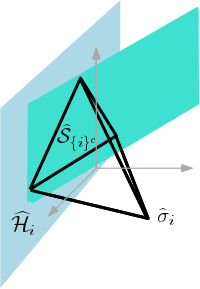
\includegraphics[scale=0.3]{Hin_plane}
		\subcaption{}
	\end{minipage}
	\begin{minipage}{0.45\textwidth}
	\centering
	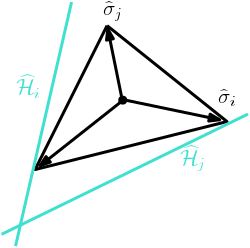
\includegraphics[scale=0.5]{Hin_plane2}
	\subcaption{}
\end{minipage}
\caption{An illustration of the fact that, in general, $\splxn_\ic$ is not contained in $\Hn_i=\{\x:\la \x,\svn_i^+\ra + \beta_i=0\}$. }
\label{fig:Hin_planes}
\end{figure}

We might expect that Lemma \ref{lem:SUn_subset} yields a hyperplane representation of the normalized simplex, as did Lemma \ref{lem:SUsubset} for the combinatorial simplex. Unfortunately however, the issue is once again complicated by the vertex weights and the relation between $\Svn^+$ and $\Svn$. Let us illustrate the problem by focusing on $\splxn$. 

As opposed to Section \ref{sec:S_G}, $\splxn_\ic $ is not contained in the hyperplane $\Hn_i = \{\x: \la \x,\svn_i^+\ra + \beta_i=0\}$, where we take $\beta_i = \beta_i^{\{i\}^c} = \sqrt{w(i)}\max_{j\neq i}\sqrt{w(j)} / \vol(G)$. To see this, take any $k\notin \argmax_{j\neq i} \sqrt{w(j)}$ (such a $k$ exists iff the graph is not regular) and note that while $\sv_k\in\splxn_U$ it is not in $\Hn_i$: 
\[\la \svn_k,\sv_i^+\ra = \bchi_k\Svn^\tp\Svn^+\bchi_i = -\frac{\sqrt{w(k)w(i)}}{\vol(G)}\neq \beta_i,\]
by assumption. The other way to see this is to note that $\svn_i^+$ is not perpendicular to $\splxn_\ic$ in general by Corollary \ref{cor:Sn_orthog_iff_regular}. Thus, it is not  clear how to generate an analogous description to Equation \eqref{eq:S_alt_desc} for the normalized simplex. While this may seem relatively inconsequential, it severely complicates finding the dual of $\splxn_G$, which is the question we turn to next. 

\paragraph{What is $\splxn_G^\du$ and and $(\splxn_G^+)^\du$?} 
Given that $\splxn_G^+$ is not the dual of $\splxn_G$ in general, it  seems appropriate  to  ask ``what on  earth \emph{is} the dual of the normalized simplex?". Somewhat surprisingly, this question is intimately related to the hyperplane representation---or lack thereof---of $\splxn_G$. 

Somewhat surprisingly, the question has a straightforward answer if we instead  ask about  $\splxn_G^+$. Using the same reasoning which was applied to $\splx_G^+$, we see that $\splxn_G^+$  is also hyperacute.
This implies, by Theorem~\ref{thm:graph-simplex}, that its centred version is the inverse \emph{combinatorial} simplex of some graph $H$. That is,  $(\splxn_G^+)_0 = \splx_H^+$. Since all translationally congruent simplices  share the same dual, we have 
\begin{equation*}
(\splxn_G^+)^\du = (\splxn_G^+)^\du_0 = (\splx_H^+)^\du = \splx_H.
\end{equation*}

\note{What's the relation between $G$ and $H$?}

We can obtain an implicit representation for the dual vertices $\{\svnd_i\}$ by noting that they must satisfy  $\la \svnd_i,\svn_j-\svn_n\ra=\delta_{ij}$ for all $i,j\neq n$. This translates to 
\begin{equation*}
\sum_{\ell=1}^n \svnd_i(\ell)(\vpn_k(j)-\vpn_k(n))\lambdan_k^{1/2}=\delta_{ij},
\end{equation*}
but extracting values of $\svnd_i$ which meet this condition is not trivial. 
We might, however, try a different tactic. Note that in the case of the combinatorial simplices, the dual vertices are encoded in their hyperplane representation by Equation \eqref{eq:S_alt_desc}: $\splx_G = \bigcap_i\{\x:\la \x,\sv_i^+\ra \geq -1/n\}$. It is thus  natural to wonder whether this relationship holds for every simplex, that is,  if given a simplex described as the intersection of haldspaces, say $\ssplx=\bigcap_i \{\x:\la \z_i,\x\ra \geq b_i\}$ are the vectors $\z_i$ are parallel to the dual vertices of $\ssplx$.  The following lemma gives gives sufficient conditions as to when this is the case. 

 
\begin{lemma}
	\label{lem:hdesc_dual}
	Let $\ssplx\subset\R^{n-1}$ be a centred simplex with $\ssplx=\bigcap_{i=1}^n  \{\x\in\R^{n-1}: \la \x,\z_i\ra \geq  \alpha_i\}$. Then $\{-\z_i/(\alpha_i n)\}$ are the vertices of $\ssplx^\du$. 
\end{lemma}
\begin{proof}
	As usual, let $\{\sv_i\}$ be the vertices of $\ssplx$. Put $\bgamma_i = -\z_i/(\alpha_i n)$. We need to show that $\{\bgamma_i\}_{i=1}^{n-1}$ is the sister basis to $\{\sv_i-\sv_n\}_{i=1}^{n-1}$. Let $H_i$ be the boundary of the halfspace $\{\x:\la \x,\z_i\ra \geq \alpha_i\}$, so $H_i = \{\x:\la \x,\z_i\ra = \alpha_i\}$. Enumerate the vertices $\{\sv_i\}$ such that $\splx_\ic \subset H_i$. Fix $i\in[n-1]$. We claim that 
	\[\sv_i \in \bigcap_{j\neq i}H_i.\]
	Indeed, $\splx_\jc$ is the $n-1$ dimensional simplex with vertices $\{\sv_\ell\}_{\ell\neq j}$. Hence $\sv_i\in \splx_\jc$ for all $j\neq i$ and thus also lies in $\cap_{j \neq i}H_j$. Therefore, $\la \sv_i,\z_j\ra = \alpha_j$ for all $j\neq i$, from which it follows  that $\la \bgamma_j,\sv_i-\sv_n\ra = -\la \z_j,\sv_i\ra/(\alpha_j n) + \la \z_j,\sv_n\ra / (\alpha_j n )=1/n - 1/n =0$.  
	It remains to show that $\la \bgamma_i,\sv_i-\sv_n\ra=1$ for all $i\neq n$. Since $\ssplx$ is centred by assumption, we have $\sv_i = -\sum_{j\neq i} \sv_j$. Consequently, 
	\begin{align*}
	\la \bgamma_i,\sv_i-\sv_n\ra &= -\sum_{j\neq i}\la \bgamma_i,\sv_j\ra - \la \bgamma_i,\sv_n \ra = \frac{1}{n}(n-1) + \frac{1}{n} = 1,
	\end{align*}
	as was to be shown.  
\end{proof}

Lemma \ref{lem:hdesc_dual} allows us to extract the dual given a hyperplane description of a centred simplex. The next natural question is then how the hyperplane description of an arbitrary simplex relates to the hyperplane description of its centred counterpart. This is answered by the following lemma. 

\begin{lemma}
	\label{lem:hdesc_centred}
	Let $\ssplx=\cap_i \{\x:\la \x,\z_i\ra \geq \alpha_i\}$ be a simplex. Its centred version, $\ssplx_0$, can be written as $\cap_i \{\x:\la \x,\z_i\ra \geq \alpha_i - \la \cent(\ssplx),\z_i\ra\}$. 
\end{lemma}
\begin{proof}
	As usual, take $\H_i = \{\x:\la \x,\z_i\ra = \alpha_i\}$ to be the hyperplanes bounding the simplex. The hyperplanes bounding the centred simplex, are parallel to the hyperplanes $\H_i$ and can thus be written as 
	\[\H_{i0} = \{\x:\la \x,\z_i\ra = \beta_i\},\]
	for some $\beta_i$. Moreover, just as $\sv_j\in\H_i$ for $j\neq i$, we have $\sv_j-\cent(\ssplx)\in \H_{i0}$, since $\{\sv_j-\cent(\ssplx)\}$ are the vertices of $\ssplx_0$. As such, $\la \sv_j-\cent(\ssplx),\z_i\ra=\beta_i$, and 
	\[\la \sv_j-\cent(\ssplx),\z_i\ra = \la \sv_j,\z_i\ra - \la\cent(\ssplx),\z_i\ra = \alpha_i - \la\cent(\ssplx),\z_i\ra,\]
	whence $\beta_i = \alpha_i - \la\cent(\ssplx),\z_i\ra$. It then follows that 
	\[\ssplx_0=\bigcap_i \H_{i0}^{\geq },\]
	where $\H_{i0}^\geq = \{\x:\la \x,\z_i\ra \geq  \alpha_i - \la \cent(\ssplx),
	\z_i\ra\}$. 
\end{proof}

Taken together, Lemmas \ref{lem:hdesc_dual} and \ref{lem:hdesc_centred} provide a path to try and determine the dual simplex of $\splxn_G$. In particular, if we could determine a hyperplane representation of any simplex congruent to $\splxn_G$,  then we can obtain a hyperplane representation of its centred version by Lemma \ref{lem:hdesc_centred} and to the dual of its centred version by Lemma \ref{lem:hdesc_dual}. Since the dual is common to all congruent simplices by Observation \ref{obs:dual_centred}, this would yield $\splx_G^\du$. The trick is simply to determine a hyperplane representation of $\splx_G$---which we leave as an exercise for the reader. Just kidding. 

 
\note{Not worth fleshing out  until we have more content for this section.}

Noting that 
\begin{equation*}
\cent(\splxn) = \frac{1}{n}\bigg(\sum_{\ell=1}^n \svn_\ell(1),\dots,\sum_{\ell=1}^n \svn_\ell(n)\bigg)^\tp,
\end{equation*}
we see that the vertices of $\splxn_0$ have coordinates
\begin{equation*}
\svn_i(j) - \cent(\splxn)(j) = \vpn_j(i)\lambdan_j^{1/2} - \frac{1}{n}\sum_{\ell=1}^n \vpn_j(\ell)\lambdan_j^{1/2} = \lambdan_j^{1/2} \bigg(\vpn_j(i) - \frac{1}{n}\la \vpn_j,\one\ra \bigg).
\end{equation*}
Likewise, the vertices of $\splxn_0^+$ have coordinates 
\begin{equation*}
\svn_i^+(j) = \evaln_j^{-1/2}\bigg(\vpn_j(i) - \frac{1}{n}\la \vpn_j,\one\ra\bigg).
\end{equation*}

Let $\cent$ be the centroid of the centred normalized Laplacian. Noting that $(\cent,\cent,\dots,\cent)=\cent\one^\tp$, 
the Gram Matrix of $\splxn_0$ is 
\begin{align*}
(\Svn-\cent\one^\tp)^\tp(\Svn-\cent\one^\tp) &= \Svn^\tp\Svn - \Svn^\tp\cent\one^\tp - \one\cent^\tp\Svn + \one\cent^\tp\cent\one^\tp \\
&= \Ln_G - \frac{1}{n} \Svn^\tp\Svn\one\one^\tp - \frac{1}{n}\one\one^\tp\Svn^\tp\Svn + \frac{1}{n^2}\Svn^\tp\Svn\one\one^\tp \\
&= \Ln_G - \frac{1}{n}\Ln_G\J - \frac{1}{n} \J\Ln_G+ \frac{1}{n^2}\J\Ln_G\J.\\
\end{align*}

\note{What are the properties of this matrix? It has an eigenvector of $\one$ with eigenvalue 0, but it does not seem to be a Laplacian. }







